\section{Vstupní data}
Vstupní data pocházejí z geodatabáze ArcČR 500 Verze 3.3, konkrétně z vrstev \texttt{silnice\_2015} a \texttt{obce\_body}.\cite{arcdataGeodatabaze}
\subsection{Načtení dat}
Tyto vrstvy byly importovány do softwaru QGIS, kde byl proveden výběr dat pro území okresu Rokycany a následný export dat do formátu GeoPackage.
\begin{itemize}
    \item \texttt{\href{https://github.com/kovarmi9/YGEI_sk3/blob/main/U3/data/roads.gpkg}{roads.gpkg}}
    \item \texttt{\href{https://github.com/kovarmi9/YGEI_sk3/blob/main/U3/data/municipalities.gpkg}{municipalities.gpkg}}
\end{itemize}
Tyto soubory byly dále načteny do Python skriptu \texttt{\href{https://github.com/kovarmi9/YGEI_sk3/blob/main/U3/convert_to_graph.py}{convert\_to\_graph.py}}, kde byla data následně zpracována za použití knihoven \texttt{\href{https://geopandas.org/}{GeoPandas}} a \texttt{\href{https://shapely.readthedocs.io/}{Shapely}} pro práci s prostorovými daty, a \texttt{\href{https://matplotlib.org/}{Matplotlib}} pro vizualizaci.

\subsection{Vizualizace dat}
Pro ověření zda byla data načtena v pořádku byly silnice a obce vizualizovány pomocí knihovny \texttt{Matplotlib}. Silniční síť byla vykreslena modře a obce červeně. Zde je ukázka silnic a obcí pro okres Rokycany:
\begin{figure}[H]
    \centering
    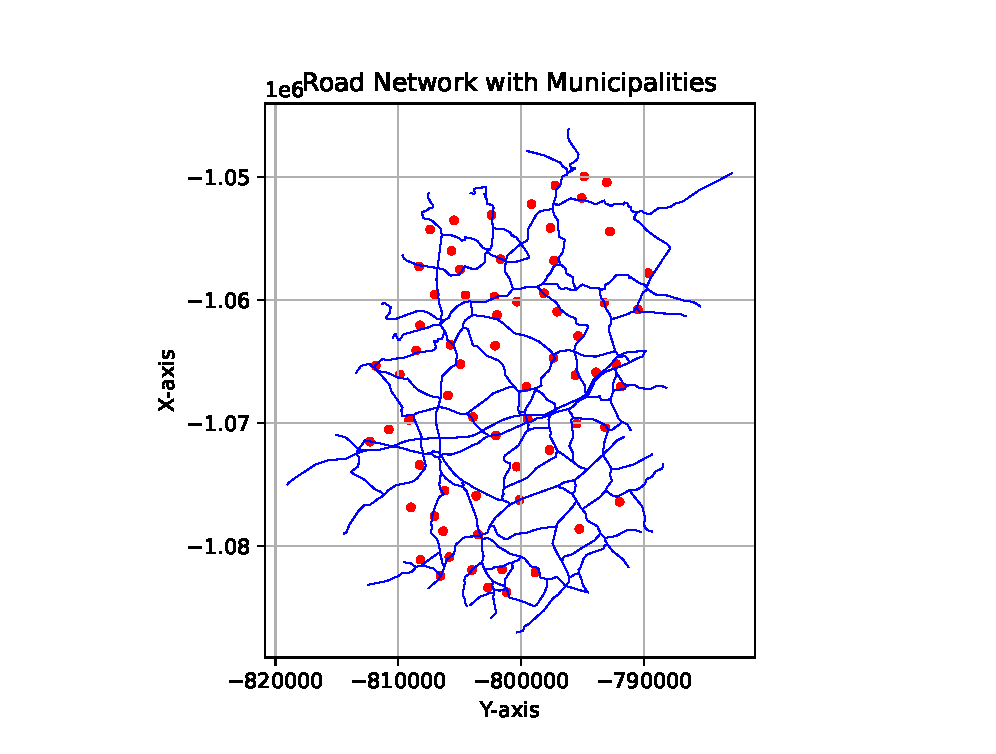
\includegraphics[width=\textwidth]{images/road_network_with_municipalities.eps}
    \caption{Silnice a obce v okrese Rokycany sloužící pro tvorbu grafu}
\end{figure}
\subsection{Výpočet dalších atributů silnic}
K jednotlivým silnicím byly přidány následující atributy:

\begin{itemize}
    \item \textbf{Délka silnice}: Délka každé silnice byla spočítána jako součet délek všech segmentů v geometrii silnice. Tento výpočet byl proveden použitím funkce \texttt{length} z knihovny \texttt{GeoPandas}, která vrací celkovou délku geometrie silnice. Tento atribut je uložen v sloupci \texttt{length}.
    
    \item \textbf{Rychlostní limit}: Každé silnici byl přiřazen rychlostní limit na základě její třídy (sloupec \texttt{TRIDA}). Tento atribut byl mapován podle předdefinovaných pravidel, kde dálnicím (\texttt{TRIDA} = 1) byl přiřazen rychlostní limit 130 km/h, rychlostním silnicím (\texttt{TRIDA} = 2) 110 km/h, silnicím 3. třídy (\texttt{TRIDA} = 3) 90 km/h, 4. třídě 70 km/h, 5. třídě 50 km/h a neevidovaným silnicím (\texttt{TRIDA} = 6) 30 km/h. Tento způsob přiřazování rychlostí neodpovídá přesně realitě, ale vzhledem k tomu, že data neobsahují informace o návrhové rychlosti, byl tento způsob zvolen jako nejvhodnější. Rychlostní limit je uložen ve sloupci \texttt{design\_speed}.
    
    \item \textbf{Zakřivení silnice}: Zakřivení silnice bylo vypočteno jako poměr celkové délky silnice, která je uložena ve sloupci \texttt{length}, a přímé vzdálenosti mezi jejím počátečním a koncovým bodem. Tento výpočet slouží k určení, jak moc je silnice klikatá.
    
    Vzorec pro výpočet zakřivení je následující:
    \[
    \texttt{curvature} = \frac{\texttt{length}}{\sqrt{(x_n - x_1)^2 + (y_n - y_1)^2}}
    \]

    kde:
    \begin{itemize}
        \item \((x_1, y_1)\) jsou souřadnice prvního bodu geometrie silnice.
        \item \((x_n, y_n)\) jsou souřadnice posledního bodu geometrie silnice.
    \end{itemize}
    
    Hodnota zakřivení poskytuje informaci o klikatost silnice:
    \begin{itemize}
        \item Pokud je zakřivení rovno 1, znamená to, že silnice je přímá (její celková délka odpovídá přímé vzdálenosti mezi počátečním a koncovým bodem).
        \item Čím vyšší je hodnota zakřivení, tím více je silnice klikatá.
    \end{itemize}
    
    Výpočet zakřivení byl implementován ve funkci \texttt{calculate\_curvature}, která iteruje přes všechny geometrie silnic v tabulce a provádí výpočet na základě výše uvedeného vzorce. Tento atribut byl následně uložen do nového sloupce \texttt{curvature}.
    
    \item \textbf{Náklady na cestu v závislosti na délce}: Tyto náklady byly spočítány jako inverzní hodnota délky silnice. Předpokládáme, že čím delší je silnice, tím vyšší jsou náklady. Tento výpočet je realizován ve sloupci \texttt{length\_weight}:
    \[
    \texttt{length\_weight} = \frac{1}{\texttt{length}}
    \]
    Tento parametr slouží k zohlednění nákladů na cestu podle délky silnice, přičemž kratší silnice mají nižší náklady.
    
    \item \textbf{Náklady na cestu v závislosti na rychlostním limitu}: Tyto náklady byly spočítány jako inverzní hodnota rychlostního limitu silnice. Předpokládá se, že silnice s vyšším rychlostním limitem umožňují rychlejší dopravu, čímž snižují náklady na cestu. Tento výpočet je implementován ve sloupci \texttt{speed\_weight}:
    \[
    \texttt{speed\_weight} = \frac{1}{\texttt{design\_speed}}
    \]
\end{itemize}

Pro ověření byly některé vypočtené hodnoty kontrolně vypsány. Ukázka dat je uvedena v tabulce:

\begin{table}[H]
    \centering
    \caption{Atributy silnic pro tvorbu grafů}
    \begin{tabular}{|c|c|c|c|c|}
    \hline
    \texttt{geometry} & \texttt{curvature} & \texttt{length\_weight} & \texttt{speed\_weight} \\
    \hline
    MULTILINESTRING ((-807558, -1083474), ...) & 1.0126 & 0.000661 & 0.014286 \\
    MULTILINESTRING ((-806520, -1082398), ...) & 1.0000 & 0.001283 & 0.014286 \\
    MULTILINESTRING ((-806220, -1081679), ...) & 1.1412 & 0.000230 & 0.014286 \\
    MULTILINESTRING ((-803307, -1079227), ...) & 1.0000 & 0.011225 & 0.014286 \\
    MULTILINESTRING ((-802511, -1078346), ...) & 1.0070 & 0.000426 & 0.014286 \\
    \hline
    \end{tabular}
\end{table}

\subsection{Zpracování silniční sítě a uzlů}
Pro každý \texttt{MultiLineString} byly extrahovány souřadnice počátečních a koncových bodů všech segmentů pomocí funkce \texttt{extract\_nodes\_from\_multilinestring}, čímž byla vytvořena sada uzlů.

\subsection{Přiřazení uzlů k obcím}
Každé obci byla přiřazena nejbližší silniční uzel na základě minimální Eukleidovské vzdálenosti. Tento výpočet byl realizován funkcí \texttt{compute\_nearest\_node}, která iteruje přes všechny obce a určuje nejbližší uzel pro jejich souřadnice. Výsledky byly uloženy do textového souboru \texttt{\href{https://github.com/kovarmi9/YGEI_sk3/blob/main/U3/data/municipalities_nearest_nodes.txt}{municipalities\_nearest\_nodes.txt}}, který obsahuje název obce a souřadnice jejího nejbližšího uzlu. Jako oddělovač je využívána čárka jelikož některé obce mají víceslovné názvy a využítí mezery jako oddělovače by vedlo k chybám. Ukázka prvních tří řádků souboru:
\begin{verbatim}
Skořice,-799379.4678585269,-1081458.7507021464
Kařízek,-791431.2708886713,-1066960.8780070543
Drahoňův Újezd,-797727.8870032951,-1059772.5634250343
\end{verbatim}

\newpage

\subsection{Export do souborů grafů}

Silniční síť byla následně převedena do formátu neorientovaného grafu, přičemž byly vytvořeny čtyři varianty reprezentace grafu podle různých kritérií vážení hran:

\begin{itemize}
    \item Graf s váhami na základě délky (\texttt{\href{https://github.com/kovarmi9/YGEI_sk3/blob/main/U3/data/graph_length_weight.txt}{graph\_length\_weight.txt}}),
    \item Graf s váhami na základě zakřivení (\texttt{\href{https://github.com/kovarmi9/YGEI_sk3/blob/main/U3/data/graph_curvature_weight.txt}{graph\_curvature\_weight.txt}}),
    \item Graf s váhami na základě rychlosti (\texttt{\href{https://github.com/kovarmi9/YGEI_sk3/blob/main/U3/data/graph_speed_weight.txt}{graph\_speed\_weight.txt}}),
    \item Nevážený graf s konstantními náklady (\texttt{\href{https://github.com/kovarmi9/YGEI_sk3/blob/main/U3/data/graph_unweighted.txt}{graph\_unweighted.txt}}).
\end{itemize}

Každý z těchto souborů obsahuje informace o jednotlivých hranách grafu, konkrétně souřadnice počátečního a koncového uzlu, a odpovídající váhu hrany. Ukázka dat z jednoho souboru je uvedena níže:
\begin{verbatim}
-807558.2415553108 -1083474.283921726 -806520.2105997838 -1082398.5459269881 1
-806520.2105997838 -1082398.5459269881 -806220.5434165187 -1081679.2349191494 1
-806220.5434165187 -1081679.2349191494 -803307.7924209237 -1079227.170260936 1
\end{verbatim}

\subsection{Načtení dat z textového souboru}

Pro načtení těchto dat z textového souboru do hlavního programu slouží \texttt{\href{https://github.com/kovarmi9/YGEI_sk3/blob/main/U3/graph\_reader.py}{graph\_reader.py}}, který umožňuje načíst data do programu z \texttt{*.txt} souborů. Konkrétně obsahuje dvě funkce pro načítání dat z textových soborů a to:

\subsubsection{Funkce pro načítání grafu}

Funkce \texttt{read\_graph} načítá data z textového souboru, který obsahuje informace o hranách grafu ve formátu:

\begin{verbatim}
x1 y1 x2 y2 w
\end{verbatim}

kde \((x1, y1)\) a \((x2, y2)\) jsou souřadnice počátečního a koncového uzlu hrany a \(w\) je váha hrany.

Tato funkce nejprve načte všechny hrany, poté vytvoří mapu bodů na identifikátory uzlů a nakonec vygeneruje samotný graf ve formě slovníku, kde každé ID uzlu ukazuje na jeho sousedy spolu s váhami hran.

\subsubsection{Funkce pro načítání názvů uzlů}

Funkce \texttt{read\_nodes\_names} načítá data z textového souboru, který obsahuje názvy obcí a jejich souřadnice ve formátu:

\begin{verbatim}
name, x, y
\end{verbatim}

Tato funkce vytváří slovník, kde klíčem je název obce a hodnotou je dvojice souřadnic \((x, y)\), které reprezentují polohu dané obce. Tento slovník je následně využíván pro přiřazení každé obci nejbližšího uzlu v grafu.

\begin{verbatim}
from graph_reader import read_graph, read_nodes_names  # Import graph loading functions

# Path to the graph file (with weights or unweighted)
file = './U3/data/graph_unweighted.txt'

# Path to the municipality file
municipalities_file = './U3/data/municipalities_nearest_nodes.txt'

# Load graph and coordinates
G, C = read_graph(file)

# Load municipalities
municipalities = read_nodes_names(municipalities_file)
\end{verbatim}

Konkrétně:

\begin{itemize}
    \item \textbf{G (graf)}: Slovník, jehož klíče představují identifikátory uzlů, přičemž každý uzel je reprezentován jako klíč ve formě čísla (ID uzlu). Hodnoty tohoto slovníku jsou další slovníky, které pro každý uzel mapují jeho sousedy (id sousedních uzlů) na váhy hran mezi nimi. Váha hrany může být například délka cesty mezi těmito uzly nebo jiný parametr (např. zakřivení nebo rychlost).
    \item \textbf{C (souřadnice)}: Slovník, který mapuje každé ID uzlu na seznam obsahující souřadnice tohoto uzlu ve formátu \([x, y]\), kde \(x\) a \(y\) jsou prostorové souřadnice uzlu v daném referenčním systému.
\end{itemize}

Příklad struktury grafu \texttt{G} a souřadnic \texttt{C} může vypadat takto:

\begin{verbatim}
# Příklad reprezentace grafu
{
    1: {2: 5.0, 3: 10.0}, # Uzel 1 je spojen s uzlem 2 váhou 5.0 a uzlem 3 váhou 10.0
    2: {1: 5.0, 3: 2.0},  # Uzel 2 je spojen s uzlem 1 váhou 5.0 a uzlem 3 váhou 2.0
    3: {1: 10.0, 2: 2.0}  # Uzel 3 je spojen s uzlem 1 váhou 10.0 a uzlem 2 váhou 2.0
}

# Příklad souřadnic (C) pro každý uzel
{
    1: [-799379.4678585269, -1081458.7507021464],# Uzel 1 a jeho souřadnice
    2: [-791431.2708886713, -1066960.8780070543],# Uzel 2 a jeho souřadnice
    3: [-797727.8870032951, -1059772.5634250343] # Uzel 3 a jeho souřadnice
}
\end{verbatim}

Kromě toho je v programu načítán soubor \texttt{municipalities\_nearest\_nodes.txt}, který obsahuje názvy obcí a souřadnice jejich nejbližších uzlů. Tento soubor je načítán funkcí \texttt{read\_nodes\_names}. Výsledkem je slovník, který mapuje názvy obcí na identifikátory uzlů grafu, na kterých se dané obce nacházejí. Struktura tohoto slovníku vypadá takto:

\begin{verbatim}
# Příklad slovníku názvů obcí a jejich nejbližších uzlů
{
    'Skořice': 1,  # Obec 'Skořice' je přiřazena k uzlu 1
    'Kařízek': 2,  # Obec 'Kařízek' je přiřazena k uzlu 2
    'Drahoňův Újezd': 3  # Obec 'Drahoňův Újezd' je přiřazena k uzlu 3
}
\end{verbatim}
